
% This LaTeX was auto-generated from MATLAB code.
% To make changes, update the MATLAB code and republish this document.

\documentclass{article}
\usepackage{graphicx}
\usepackage{color}

\sloppy
\definecolor{lightgray}{gray}{0.5}
\setlength{\parindent}{0pt}

\begin{document}

    
    \begin{verbatim}
n=[10,30,50];
theta=2.2;
Counter=1;
dimN=size(n,2);

MLEStats=zeros(dimN,3);

while Counter<=dimN
    %Calculates random variables for different sample sizes
    data=zeros(n(Counter),200);
    mle_data=zeros(1,200);
    count=1;
    while count<=200
        u=rand(n(Counter),2);
        x=-log(1-u(:,1))/theta-log(1-u(:,2))/theta;
        data(:,count)=x;
        mle_data(1,count)=2*n(Counter)/sum(x);
        count=count+1;
    end

    %Calculating Average and Varience in data
    MLEStats(Counter,1)=sum(mle_data)/200;
    var_mle=0;
    weight_var_mle=0;
    count=1;
    while count<=200
        var_mle=var_mle+(mle_data(1,count)-MLEStats(Counter,1))^2;
        weight_var_mle=weight_var_mle+(mle_data(1,count)-theta)^2;
        count=count+1;
    end
    MLEStats(Counter,2)=var_mle/200;
    MLEStats(Counter,3)=weight_var_mle/200;

    if Counter==1
        XLower=min(mle_data)-0.2;
        XHigher=max(mle_data)+0.2;
    end

    %Plots histogram with appropiate data
    figure
    histogram(mle_data,'Normalization','pdf')
    xlim([XLower,XHigher])
    hold on
    line([theta,theta],ylim,'LineWidth', 2,...
        'Color', 'r');
    hold on
    x=linspace(XLower,XHigher);
    y=pdf(x,2*n(Counter),theta);
    line(x,y,'LineWidth',2,'Color','g')

    legend('Data','\theta_{0}=2.2','Exact p.d.f','Location','northeast')
    xlabel('M.L.E')
    ylabel('Frequency Density')
    print(strcat('Image_8_',num2str(Counter)),'-depsc')

    Counter=Counter+1;
end
%MLE denotes average mle | Variance from average mle | Variance from 2.2
disp(MLEStats)
latex(sym(vpa(MLEStats)))

function answer = pdf(x,a,b)
    answer=(a*b)^(a)./((gamma(a)).*(x.^(a+1))).*exp(-b.*a./x);
end
\end{verbatim}

        \color{lightgray} \begin{verbatim}          2.27616722689254         0.293039143016677         0.298840589469177
          2.24671917673426          0.07780028178815         0.079982963262877
          2.19116586559219        0.0507181125009796        0.0507961544317149


ans =

    '\left(\begin{array}{ccc} 2.27616722689254391553959067096 & 0.29303914301667716157950849265035 & 0.29884058946917746446558794559678\\ 2.2467191767342602481960511795478 & 0.077800281788149974748769466259546 & 0.079982963262876974330772839039128\\ 2.1911658655921892879803181131138 & 0.050718112500979600776318534371967 & 0.05079615443171485444917578888635 \end{array}\right)'

\end{verbatim} \color{black}
    
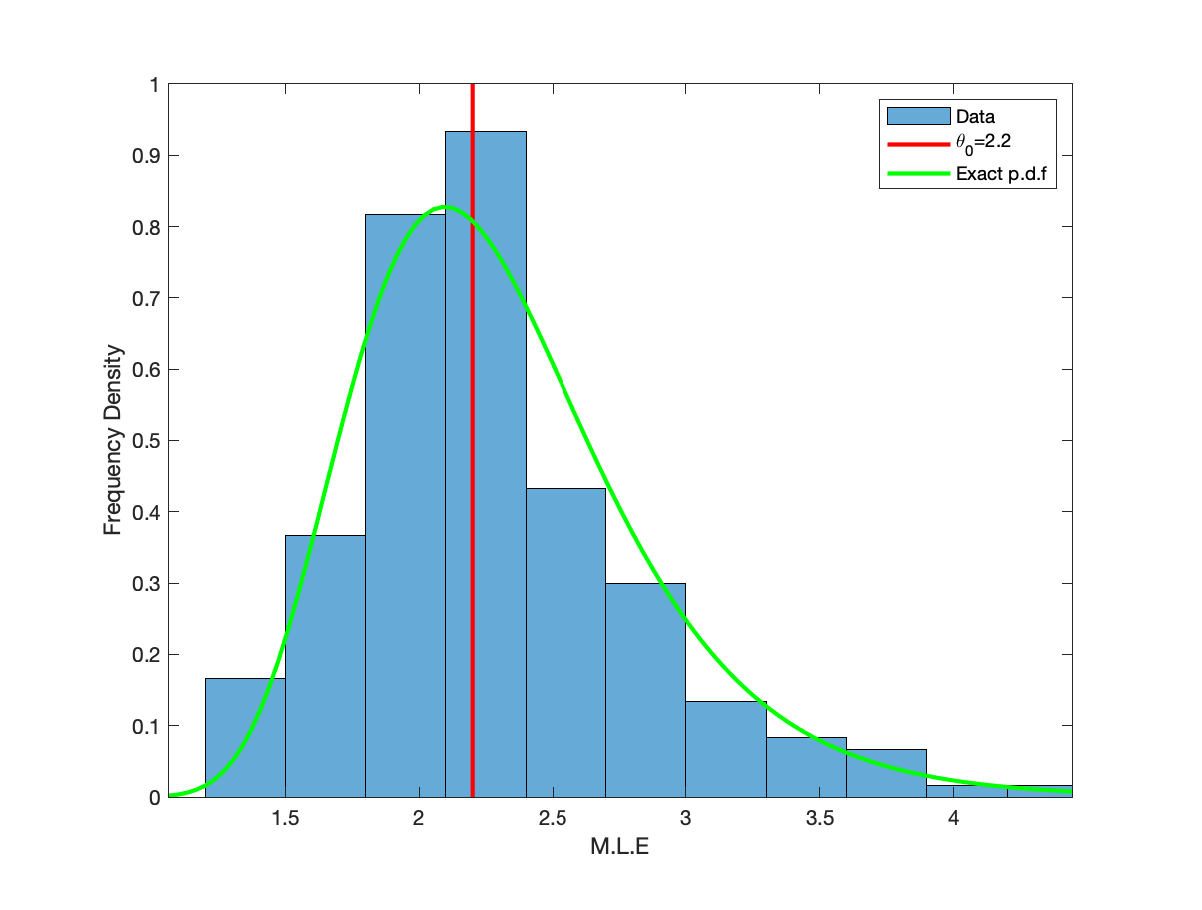
\includegraphics [width=4in]{Code_8_1_01.eps}

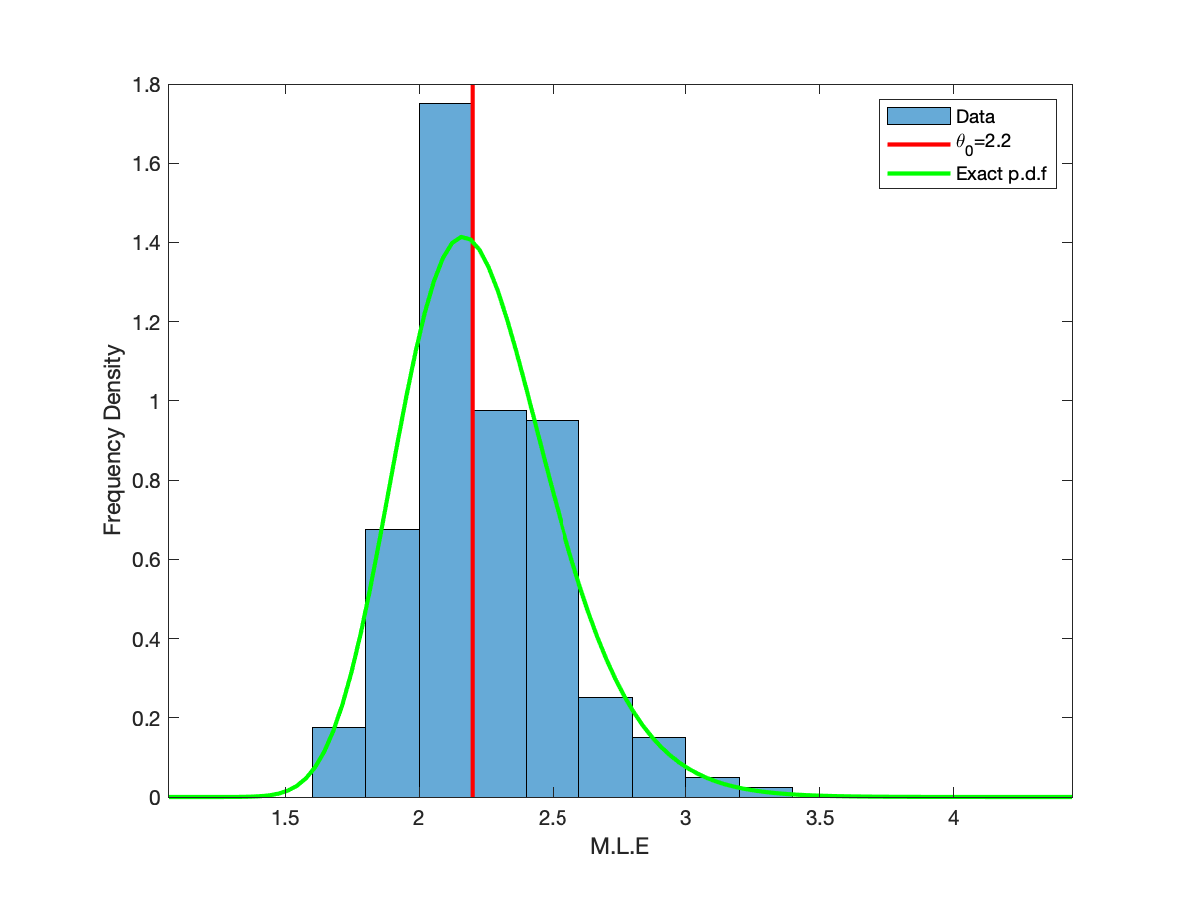
\includegraphics [width=4in]{Code_8_1_02.eps}

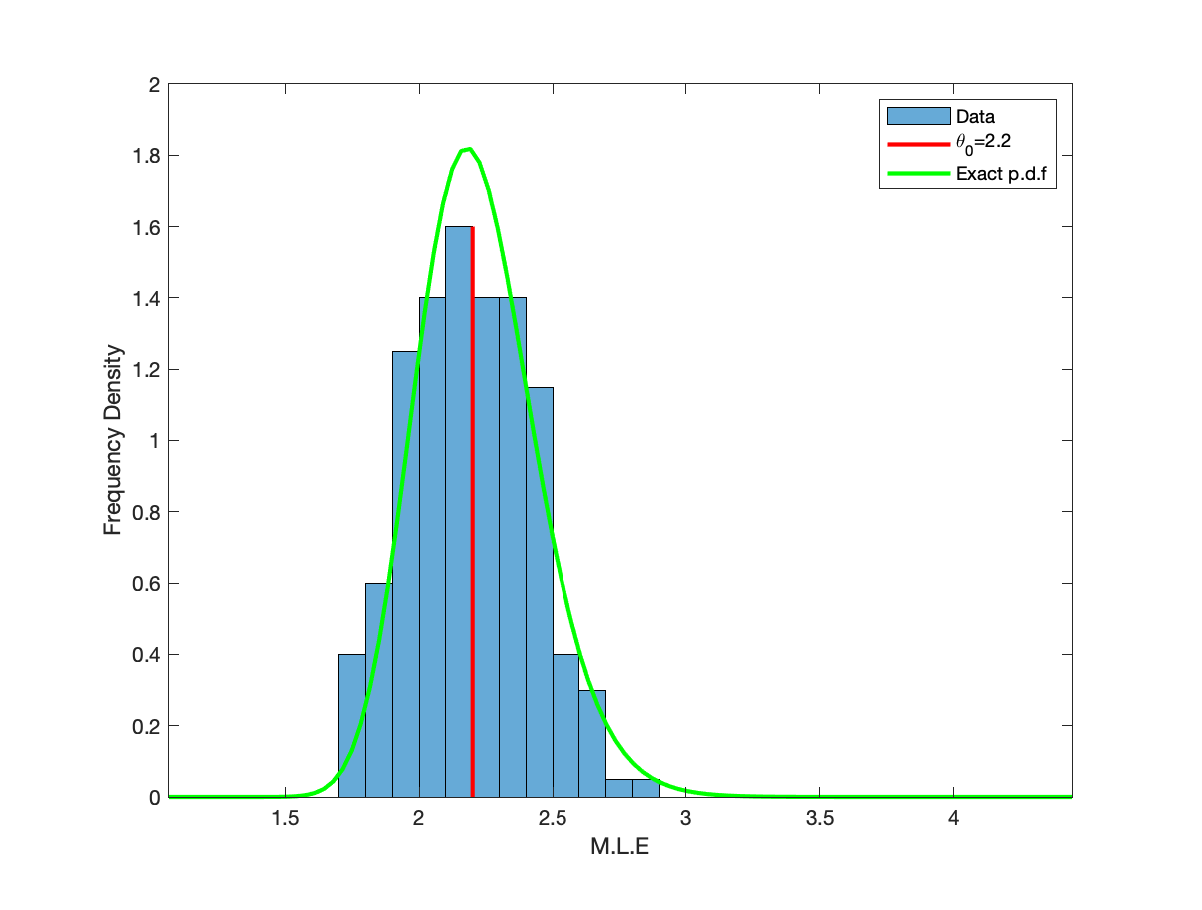
\includegraphics [width=4in]{Code_8_1_03.eps}



\end{document}
    
